\documentclass[answers]{exam}
\usepackage{texPreamble}
\usepackage{relsize}
\usepackage{tabularx}
\extraheadheight{0.25in}
\extrafootheight{1.0in}
\extrawidth{1in}
% ----------------------------------------------------------------

\begin{document}
%\relscale{1.4}
\section{2.7: Precise Definition of Limits}

\begin{defn*}[Limit of a Function]
  Assume $f(x)$ is defined for all $x$ in some open interval containing $a$, except possibly at $a  $. We say \textbf{the limit of $\bm{f(x)}$ as $\bm x$ approaches $\bm a$ is $\bm L$}, written 
    $$\lim_{x \to a} f(x)=L$$
  if for \textit{any} number $\eps>0$ there is a corresponding number $\delta>0$ such that
  {\setlength{\belowdisplayskip}{0pt}
    $$\abs{f(x)-L}<\eps\text{ whenever } 0<\abs{x-a}<\delta$$}
  \vspace*{-20pt}
\end{defn*}

\noindent
  If we know $L$ and $\eps>0$ is given, we can draw horizontal lines $L-\eps$ and $L+\eps$. Using the intersections of the graph and the horizontal lines, we can solve for $\delta>0$ such that for values of $x$ in the interval $(a-\delta,a+\delta),\ x\neq a$, we have $L-\eps\leq f(x)\leq L+\eps$.
\vspace*{-5pt}

\begin{center}
  \begin{tikzpicture}[scale=0.77]
    \begin{groupplot}[
      group style={group size=3 by 1, horizontal sep=1.25cm},
      axis lines=center,
      axis line style={->},
      xmin=0, xmax=4,
      ymin=0, ymax=4,
      xtick={2.675},
      ytick={2.9429},
      xticklabels={$a$},
      yticklabels={$L$},
      enlargelimits={abs=0.65},
      ticklabel style={font=\large, inner sep=0.75pt,fill=white},
      every axis plot/.append style={line width=0.95pt}
      ]
    \nextgroupplot
      \addplot[-] expression[domain=1.575:3.865, blue] {cot(deg(x-pi/3))+3)};
      \draw[dashed, line width=0.75pt] (axis cs: 0,2.9429) -- (axis cs: 2.675,2.9429) -- (axis cs:2.675,0);
    \nextgroupplot[
      xtick={2.675},
      ytick={1.7853,2.9429,3.9658},
      xticklabels={$a$},
      yticklabels={$L-\eps$,$L$,$L+\eps$},
      ]
      \fill[fill=ClemsonPurple, opacity=0.25] (axis cs:0,1.7853) rectangle ++(6,2.1805);
      \addplot[-] expression[domain=1.575:3.865, blue] {cot(deg(x-pi/3))+3)};
      \draw[dashed, line width=0.5pt] (axis cs: 0,1.7853) -- (axis cs: 6,1.7853);
      \draw[dashed, line width=0.5pt] (axis cs: 0,3.9658) -- (axis cs: 6,3.9658);
      \draw[dashed, line width=0.75pt] (axis cs: 0,2.9429) -- (axis cs: 2.675,2.9429) -- (axis cs:2.675,0);
    \nextgroupplot[
      xtick={1.85,2.675,3.5},
      ytick={1.7853,2.9429,3.9658},
      xticklabels={$a-\delta$,$a$,$a+\delta$},
      yticklabels={$L-\eps$,$L$,$L+\eps$},
      ]
      \fill[fill=ClemsonOrange, opacity=0.25] (axis cs:1.85,0) rectangle ++(1.65,6);
      \fill[fill=ClemsonPurple, opacity=0.25] (axis cs:0,1.7853) rectangle ++(6,2.1805);
      \addplot[-] expression[domain=1.575:3.865, blue] {cot(deg(x-pi/3))+3)};
      \draw[dashed, line width=0.5pt] (axis cs: 1.85,0) -- (axis cs: 1.85,6);
      \draw[dashed, line width=0.5pt] (axis cs: 3.5,0) -- (axis cs: 3.5,6);
      \draw[dashed, line width=0.5pt] (axis cs: 0,1.7853) -- (axis cs: 6,1.7853);
      \draw[dashed, line width=0.5pt] (axis cs: 0,3.9658) -- (axis cs: 6,3.9658);
      \draw[dashed, line width=0.75pt] (axis cs: 0,2.9429) -- (axis cs: 2.675,2.9429) -- (axis cs:2.675,0);
    \end{groupplot}
  \end{tikzpicture}
  
  \textit{Note:} As $\eps$ becomes smaller, $\delta$ will become smaller as well.
\end{center}
\vspace*{-15pt}
\hrulefill

\begin{ex*}
  Use the graph of $f$ below to find a number $\delta$ such that if $0<\abs{x-2.25}<\delta$ then $\abs{f(x)-2.159}<1$.
\end{ex*}  
\vspace*{-20pt}
\begin{flushright}
  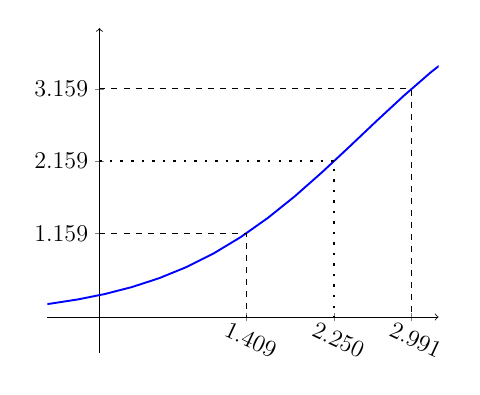
\begin{tikzpicture}[scale=0.725]
    \begin{axis}[
      axis lines=center,
      axis line style={->},
      xmin=-0.5, xmax=3.25,
      ymin=-0.5, ymax=4,
      xtick={1.409,2.25,2.991},
      xticklabels={1.409,2.250,2.991},
      ytick={1.159,2.159,3.159},
      yticklabels={1.159,2.159,3.159},
      xticklabel style={font=\large, rotate=-25, yshift=5pt},
      yticklabel style={font=\large},
      every axis plot/.append style={line width=0.95pt}
      ]
      \addplot[-] expression[domain=-1.25:5, blue] {5/(1+3^(2.5-x))};
      \draw[dashed] (axis cs: 0,1.159) -- (axis cs: 1.409,1.159) -- (axis cs: 1.409,0);
      \draw[dashed] (axis cs: 0,3.159) -- (axis cs: 2.991,3.159) -- (axis cs: 2.991,0);
      \draw[loosely dotted, line width=1.25pt] (axis cs: 0,2.159) -- (axis cs: 2.25,2.159) -- (axis cs: 2.25,0);
    \end{axis}
  \end{tikzpicture}
\end{flushright}
\vspace*{-15pt}
\pagebreak
\begin{ex*}
  Use the graph of $g(x)=\sqrt x+1$ to help find a number $\delta$ such that if $\abs{x-4}<\delta$ then $\ds\abs{\parens{\sqrt x+1}-3}<\frac{1}{2}$.
  \vspace*{-25pt}
  \begin{flushright}
    \begin{tikzpicture}
      \begin{axis}[
        axis lines=center,
        axis line style={->},
        xmin=-0.25, xmax=7.25,
        ymin=-0.25, ymax=4.5,
        xtick={2.25,4,6.25},
        xticklabels={$x_1$,4,$x_2$},
        ytick={2.5,3,3.5},
        ticklabel style={font=\large, inner sep=0.75pt},
        every axis plot/.append style={line width=0.95pt}
        ]
        \addplot[-] expression[blue, samples at={0,0.05,...,7.25}] {sqrt(x)+1};
        \draw[dashed] (axis cs: 0,2.5) -- (axis cs: 2.25,2.5) -- (axis cs: 2.25,0);
        \draw[dashed] (axis cs: 0,3.5) -- (axis cs: 6.25,3.5) -- (axis cs: 6.25,0);
        \draw[loosely dotted, line width=1.25pt] (axis cs: 0,3) -- (axis cs: 4,3) -- (axis cs: 4,0);
      \end{axis}
    \end{tikzpicture}
  \end{flushright}
\end{ex*}
\vspace{\stretch{1}}
\begin{ex*}
  Use the graph of the following linear function where $\ds\lim_{x \to 3} h(x)=5$ to find $\delta>0$ such that $\abs{h(x)-5}<1$ whenever $0<\abs{x-3}<\delta$.
  \begin{flushright}
    \begin{tikzpicture}
      \begin{axis}[
        axis lines=center,
        axis line style={->},
        grid=both,
        grid style={line width=0.35pt, draw=gray!75},
        xmin=-0.25, xmax=7.25,
        ymin=-0.25, ymax=7.25,
        xtick={0,1,...,7},
        ytick={0,1,...,7},
        ticklabel style={font=\large, inner sep=0.75pt},
        every axis plot/.append style={line width=0.95pt}
        ]
        \fill[color=ClemsonOrange, opacity=0.25] (axis cs:0,4) rectangle (axis cs: 8,6);
        \draw[dashed] (axis cs: 0,4) -- (axis cs: 8,4);
        \draw[dashed] (axis cs: 0,6) -- (axis cs: 8,6);
        \addplot[-] expression[blue, domain=-0.25:7.25] {0.5*x+3.5};
      \end{axis}
    \end{tikzpicture}
  \end{flushright}
\end{ex*}
\pagebreak
\noindent
\fbox{\parbox{\linewidth}{\textbf{Steps for proving that $\ds\lim_{x \to a} f(x)=L$}
  \begin{enumerate}
    \item \textbf{Find }$\bm \delta.$ Let $\eps$ be an arbitrary positive number. Use the inequality $\abs{f(x)-L}<\eps$ to find a condition of the form $\abs{x-a}<\delta$, where $\delta$ depends only on the value of $\eps$.
    \item \textbf{Write a proof.} For any $\eps>0$, assume $0<\abs{x-a}<\delta$ and use the relationship between $\eps$ and $\delta$ found in Step 1 to prove that $\abs{f(x)-L}<\eps$.
  \end{enumerate}
  }}
  
  \begin{ex*}
    Use the $\eps-\delta$ definition of a limit to prove $\ds\lim_{x \to 4}(2x-5)=3$.
    \vspace*{\stretch{1}}
  \end{ex*}
  \begin{ex*}
    Use the $\eps-\delta$ definition of a limit to prove $\ds\lim_{x \to 2}\dfrac{x}{5}=\dfrac{2}{5}$.
    \vspace*{\stretch{1}}
  \end{ex*}
  \pagebreak
  \begin{ex*}
    Use the $\eps-\delta$ definition of a limit to prove $\ds\lim_{x \to 2}\dfrac{x^2+x-6}{x-2}=5$.
    \vspace*{\stretch{1}}
  \end{ex*}
  \begin{ex*}
    Use the $\eps-\delta$ definition of a limit to prove $\ds\lim_{x \to 3}\dfrac{x^2+2x-15}{2x-6}=4$.
    \vspace*{\stretch{1}}
  \end{ex*}
  \pagebreak
\end{document}
